\chapter[Modular Synthesizer]{Building a Virtual Analog Modular Synthesizer}\label{chapter:building-a-mod-synth}

%https://www.gemtracks.com/guides/view.php?title=music-genres-and-their-typical-bpms&id=823 -> cite for SuperCollider tempo module
%http://hyperphysics.phy-astr.gsu.edu/hbase/Music/mussca.html -> for arpeggiator module, on how to decide how to dynamically get the third and fifth intervals -> also need to explain interval ratios

\section{Building the GUI}\label{section:building-the-gui}

\section{The Modules: Pure Waveforms}

The waveforms created through SuperCollider are through the ``SinOsc'' Unit Generator. As in Listing \ref{lst:sinewave-synthdef}, a simple sine wave is created, with a frequency of 440 Hz, and a volume of 50. Thus, as previously seen in both Figure \ref{fig:basic-sine-wave} and Equation \ref{eq:sine-wave-equation}, a continuous sine wave has been created.

\begin{listing}
	\begin{lstlisting}
		SynthDef("sinewave", {arg freq=440, vol=50; Out.ar(0, SinOsc.ar(freq, 0, vol))}).add;
	\end{lstlisting}
	\caption{Creating a sine wave SynthDef in SuperCollider}
	\label{lst:sinewave-synthdef}
\end{listing}

\begin{listing}
	\begin{lstlisting}
		x = Synth("sinewave");
	\end{lstlisting}
	\caption{Putting the sine wave SynthDef into a Synth, for sound output}
	\label{lst:sinewave-synth}
\end{listing}

\subsection{Volume Slider}

Volume is a simple concept to understand, as it is how loud or soft the human ear hears at a particular frequency. Volume ranges, as they are known in classical music, begins at a soft, and at times, barely audible \textit{pianissimo}, and become as loud as \textit{fortissimo}. The sine wave SynthDef created in Listing \ref{lst:sinewave-synthdef} contains a variable value for volume. In the SynthDef, the volume is initialized at the number 50, which generally correlates to a medium-loud volume of \textit{mezzo forte}.

As the sine wave Synth Def contains two variables, one for frequency, and one for volume, creating modules for both a volume slider and a pitch knob is simple. To create the volume slider, a SuperCollider class called \textit{EZSlider}, which creates the outline of the volume slider itself, as in Figure \ref{fig:volume-slider-basic}. For the slider's functionality, there are three important parts: the ``controlSpec,'' ``action,'' and ``initVal.'' The ``controlSpec'' defines the ``control spec,'' or the range of values allowed for the specified module. Negative volume does not exist, so this simple volume module will contain valid values for 0 volume (\textit{pianissimo}) up to 100 volume (\textit{fortissimo}). Then, the ``action'' argument of the \textit{EZSlider} class determines the function that runs when the value of the volume slider is changed. 

\begin{figure}[h]
  \centering
  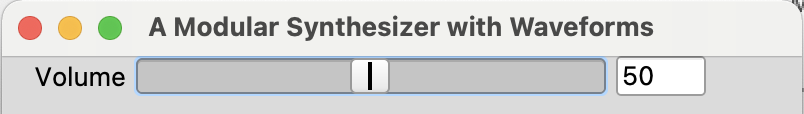
\includegraphics[width=\textwidth]{volume-slider-basic.png}
  \caption{The basic volume slider, with a volume of 50, or \textit{mezzo forte}}
  \label{fig:volume-slider-basic}
\end{figure}

\begin{listing}
	\begin{lstlisting}
		volumeSlider = EZSlider(awindow, label:"Volume", controlSpec:[0,100], action:{|mv| x.set("vol", mv.value)}, initVal:50);
	\end{lstlisting}
	\caption{Creating the volume slider in SuperCollider}
	\label{lst:volume-slider-waveform}
\end{listing}

In Listing \ref{lst:volume-slider-waveform}, the action that is set involves changes to the Synth that was created in Listing \ref{lst:sinewave-synth}. In this code example, the SynthDef from Listing \ref{lst:sinewave-synthdef} that is assigned to the variable name ``sinewave'' is now put into a Synth. This Synth, as previously described, allows SuperCollider to deal with audio output. So, the SynthDef ``sinewave'' is put into a Synth, known as ``x.'' Within the action, $x$ is able to be manipulated, that is the sine wave which is in the Synth can be manipulated, resulting in an altered sound. The action itself begins with a reference to the volume slider itself, $mv$. The Synth $x$ then references the volume argument from the SynthDef, ``vol,'' which sets the volume for both the SynthDef and the Synth, and uses the \texttt{set} function to set the volume of the Synth equal to the volume that the volume slider contains. The volume of the Synth $x$ will update as the value of the volume slider does, setting the value of \texttt{x.vol} to be equivalent to \texttt{mv.value}. Finally, ``initVal'' simply initializes the starting value of the slider to volume 50 (\textit{mezzo forte}).

\subsection{Pitch Knob: The Pitch Bend}

Pitch, as previously mentioned, is simply a functionality which dictates the frequency of a note that the human ear perceives. Standard Western tuning currently dictates notes to be tuned around the starting pitch of the note A above Middle C (or $A_5$), which is equivalent to 440 Hz. In Listing \ref{lst:sinewave-synthdef}, we notice that the sine wave SynthDef is created, with two arguments: the frequency for the sine wave to play at, and the volume of the sine wave. The frequency of the sine wave that is created is equivalent to the variable \textit{B} in the generic sine wave equation (Equation \ref{eq:sine-wave-equation}).

Similar to the volume slider, creating the pitch knob in SuperCollider relies on the use of a native class, \textit{EZKnob}. This class creates the knob, as in Figure \ref{fig:pitch-wheel-basic}. Like with the class \textit{EZSlider}, the knob also has the ``controlSpec,'' ``action,'' and ``initVal.'' The controlSpec for the pitch knob is \texttt{freq}, denoting the span of available frequencies, of the valid notes within standard tuning systems. While negative frequency values do not exist, valid frequency values would exist within the human range of hearing (that is, 20 Hz to 20 kHz). The ``action'' argument works similarly to its functionality in the volume slider, as it sets the \texttt{freq} argument of SynthDef ``sinewave'' equal to the frequency value of the pitch knob. Then, the Synth of Listing \ref{lst:sinewave-synth}, ``x,'' continuously matches the value of the pitch knob (\texttt{mn.value}) to the frequency value of the SynthDef, and thus also the Synth. The final argument of the \textit{EZKnob} class is ``initVal,'' in which the initial value of the pitch knob is set to 440 Hz.

\begin{figure}
  \centering
  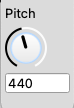
\includegraphics{pitch-wheel-basic.jpg}
  \caption{The basic pitch wheel, with a pitch of 440 Hz, or $A_5$}
  \label{fig:pitch-wheel-basic}
\end{figure}

\begin{listing}
	\begin{lstlisting}
		pitchKnob = EZKnob(awindow, label:"Pitch", controlSpec:\freq, action:{|mn| x.set("freq", mn.value)}, initVal:440);
	\end{lstlisting}
	\caption{Creating the pitch knob in SuperCollider}
	\label{lst:pitch-knob-waveform}
\end{listing}



\subsection{Legato Switch: A Sustain Button}

The \textit{legato} switch for this synthesizer is meant to emulate the legato notation found in classical music. Legato is a directive, typically found in its full form in classical music, which indicates the performance of a specific passage to be played in a smooth, graceful, and connected style (opposed to the \textit{staccato} notation) \cite{Winer_2018}. It will often be indicated by a slur over the notes, or an accent mark with a line over the notes to be affected, as in Figure \ref{fig:legato-example}\cite{Henle_2009}. On a physical electronic keyboard, this module is most often seen with a \textit{sustain} button, in which the notes played are extended, and slurred into each other. However, it is important to note that not all slur lines in written sheet music will be meant to be played legato. Notes that are to be played legato will differ in pitch, connecting notes of different pitches to be played in succession in a smooth manner. This is unlike the notation for tied notes, as in Figure \ref{fig:tied-notes-example}\cite{Lung_2016}, which connect notes that are the same pitch. The durations of the notes which are tied together are combined, and played at that new longer note duration instead. However, further development on this module is not needed. A continuous sine wave was created through the SynthDef, and later put into a Synth for sound output. A module which sustains a note, or in the case a waveform, and smoothly connects it to the next waveform will not alter the sound of the continuous waveforms that are created within SuperCollider code.

\begin{figure}[h]
  \centering
  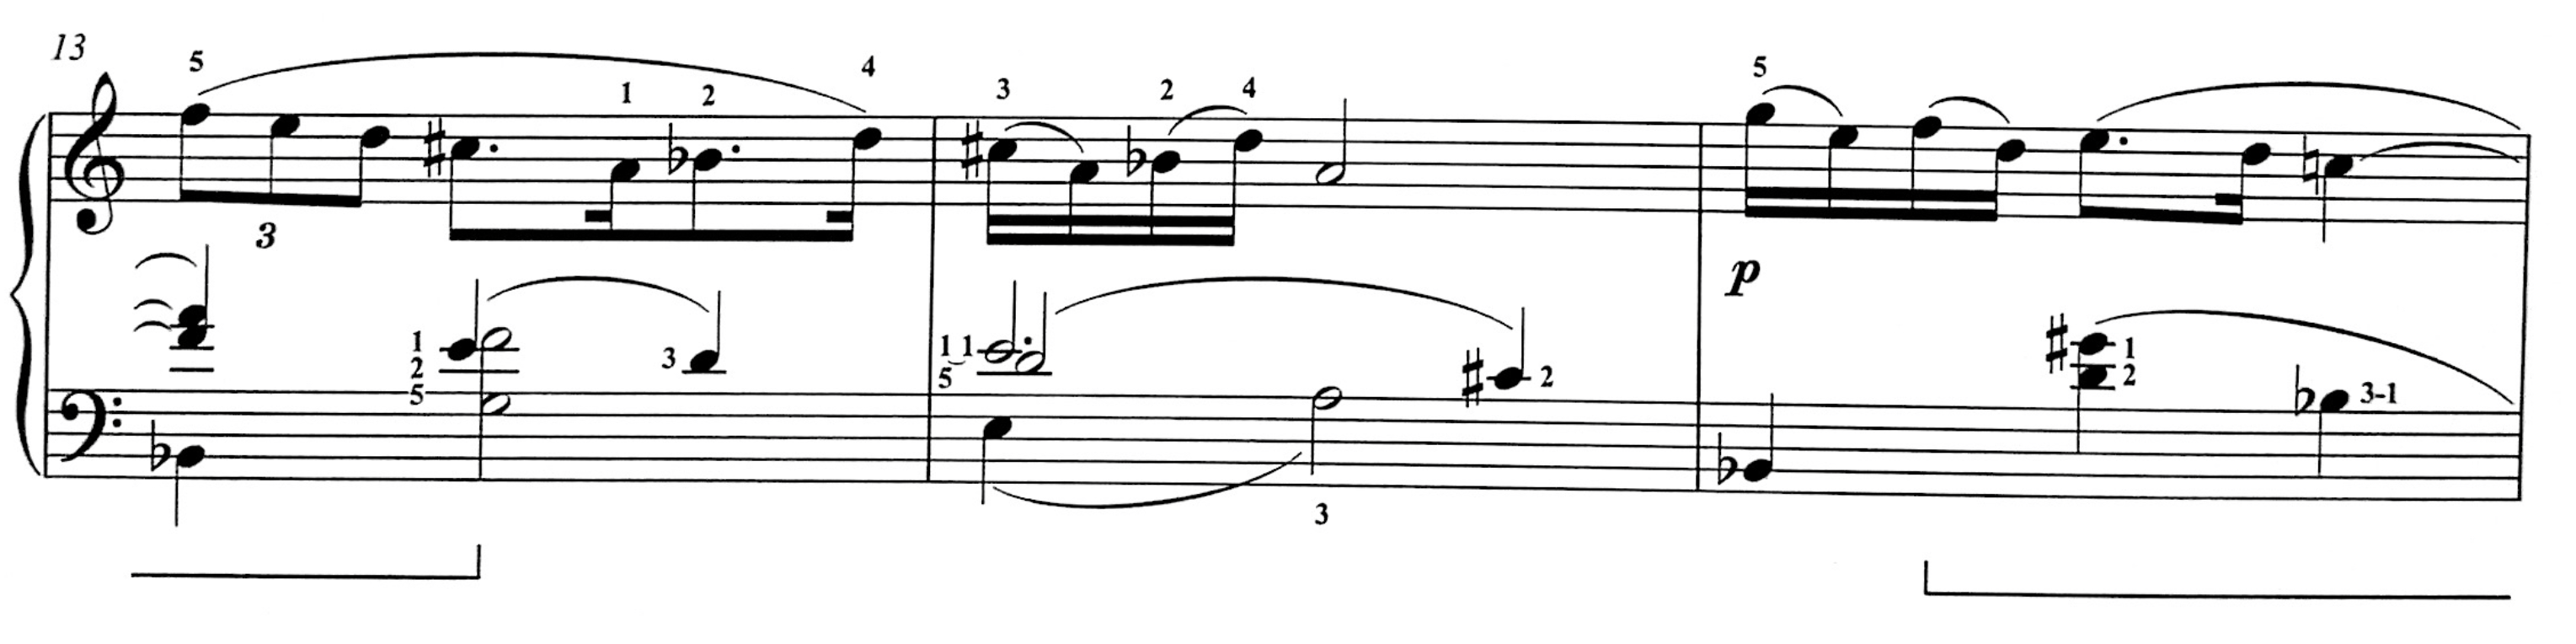
\includegraphics[width=\textwidth]{bartok-dance-four-b-section-second-system.jpg}
  \caption{An example of legato notation, found in Bela Bartok's \textit{Six Romanian Folk Dances}, Sz. 56, BB 68}
  \label{fig:legato-notes-example}
\end{figure}

\begin{figure}[h]
  \centering
  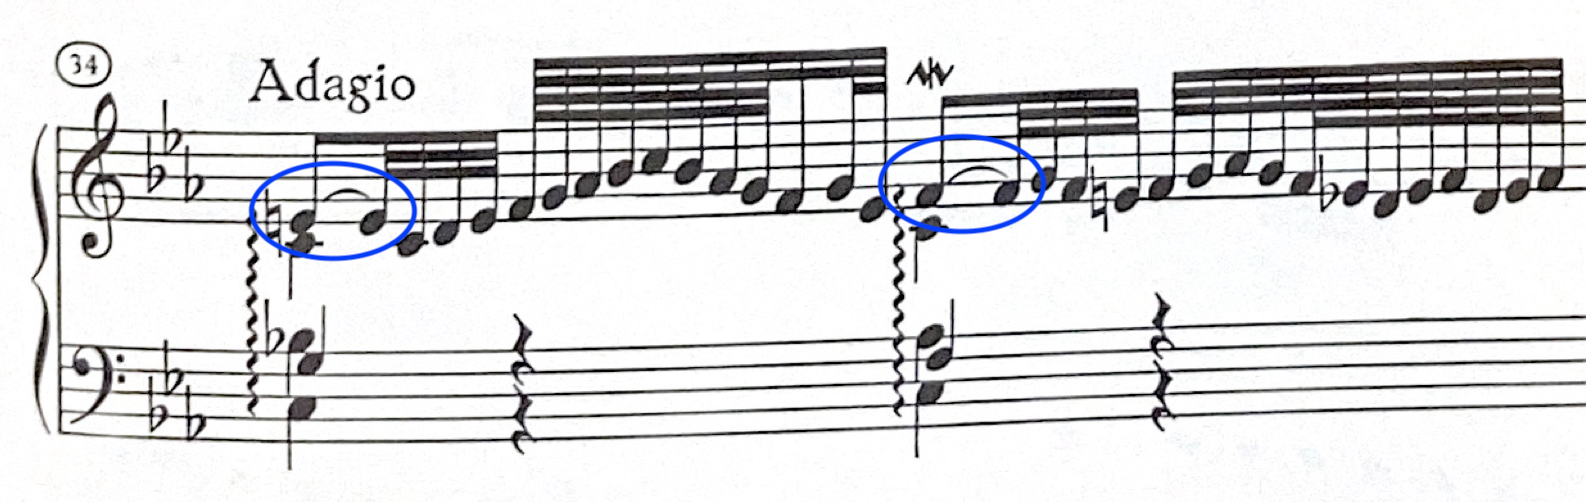
\includegraphics[width=\textwidth]{bach-prelude-second-motive.jpg}
  \caption{An example of tied notes, found in J.S. Bach's \textit{Prelude in C Minor}, from \textit{The Well-Tempered Clavier, Book I}, BVW 847}
  \label{fig:tied-notes-example}
\end{figure}

\subsection{}

\section{MIDI Input}\label{section:midi-input}
% how MIDI is input in SuperCollider

\section{The Modules: In Midi}\label{section:the-modules-midi}
% how the MIDI input was changed

\subsection{Pitch Bend}